\begin{thm}{203}{\hosi 6}{第二回駿台全国 (2017)}
 半径$R$の外接円Kを持つ正三角形ABCと、Kの劣弧AB上(ただし両端を除く)に点Pがあり、$\angle\mr{PCB}=\theta$とするとき、$\mr{PA}+\mr{PB}^2+\mr{PC}$を$R, \theta$を用いて表せ。またPが劣弧AB上(ただし両端を含む)を動くとき、$\mr{PA}+\mr{PB}^2+\mr{PC}$の最大値を求めよ。
\end{thm}

\begin{wrapfigure}[10]{r}[0pt]{100pt}
 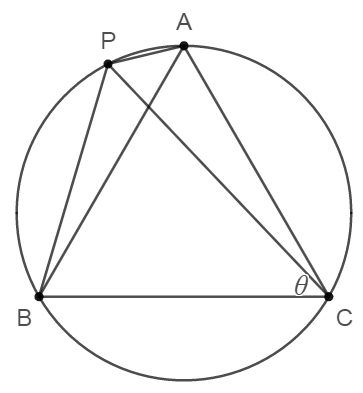
\includegraphics[width=\linewidth]{../problems/Q_203/A_203.png}
\end{wrapfigure}
両端を除く劣弧AB上を点Pが動くとき、$\theta$は$0<\theta<\dfrac{\pi}{3}$の範囲を動く。$\triangle\mr{PCB}$の外接円もKに等しいから、正弦定理によって、$\mr{PB}=2R\sin\theta$。$\angle\mr{PCA}=\dfrac{\pi}{3}-\theta$であることを用いて、正弦定理によって$\mr{PA}=2R\sin\left(\dfrac{\pi}{3}-\theta\right)$。円周角の定理より$\angle\mr{PCB}=\angle\mr{PAB}$なので、$\angle\mr{PAC}=\dfrac{\pi}{3}+\theta$であるから、正弦定理によって$\mr{PC}=2R\sin\left(\dfrac{\pi}{3}+\theta\right)$。これらによって、
\begin{align*}
 &\mr{PA}+\mr{PB}^2+\mr{PC} \\
 =&2R\sin\left(\frac{\pi}{3}-\theta\right)+\bigl(2R\sin\theta\bigr) + 2R\sin\left(\frac{\pi}{3}+\theta\right) \\
 =& 4R^2\sin^2\theta+2\sqrt{3}R\cos\theta \quad \text{(*)}
\end{align*}
と求まった。

点Pが点A, Bに重なる場合も、それぞれ$\theta=\dfrac{\pi}{3}, 0$とすれば(*)は成り立つ。よって$0\le\theta\le\dfrac{\pi}{3}$の範囲で考える。$\cos\theta=t$とおけば、$\dfrac{1}{2}\le t\le 1$であって(*)は
\begin{align*}
 \mr{PA}+\mr{PB}^2+\mr{PC}&=4R^2(1-t^2)+2\sqrt{3}Rt \\
 &=-4R^2\left(t-\frac{\sqrt{3}}{4R}\right)^2+4R^2+\frac{3}{4}
\end{align*}
これの最大値について考える。

(i)~$\dfrac{\sqrt{3}}{4R}<\dfrac{1}{2}$すなわち$R>\dfrac{\sqrt{3}}{2}$のとき、$t=\dfrac{1}{2}$において最大値$3R^2+\sqrt{3}R$をとる。

(ii)~$\dfrac{1}{2}\le \dfrac{\sqrt{3}}{4R}\le 1$すなわち$\dfrac{\sqrt{3}}{4}\le R\le \dfrac{\sqrt{3}}{2}$のとき、$t=\dfrac{\sqrt{3}}{4R}$において最大値$4R^2+\dfrac{3}{4}$をとる。

(iii)~$1<\dfrac{\sqrt{3}}{4R}$すなわち$0<R<\dfrac{\sqrt{3}}{4}$のとき、$t=1$において最大値$2\sqrt{3}R$をとる。

以上まとめて最大値は、
\begin{align*}
 \left\{
 \begin{aligned}
  &3R^2+\sqrt{R} & &\left(\frac{\sqrt{3}}{2}<R\right) \\
  &4R^2+\frac{3}{4} & &\left(\frac{\sqrt{3}}{4}\le R\le \frac{\sqrt{3}}{2}\right) \\
  &2\sqrt{3}R & &\left(0<R<\frac{\sqrt{3}}{4}\right)
 \end{aligned} \right.
\end{align*}
